\chapter{Superficies, adsorción y catálisis heterogénea}\label{ch:b3:surfaces-catalysis}

Bajo un coche, dentro de una carcasa de acero, hay un panal cerámico cuyos miles de
canales están recubiertos de un óxido poroso que retiene unos pocos gramos de platino,
paladio y rodio. En una fracción de segundo, los gases de escape que lo
atraviesan pierden la mayor parte de su monóxido de carbono, de sus hidrocarburos sin quemar y
de sus óxidos de nitrógeno. Nada ocurre en el gas: cada una de estas reacciones tiene
lugar en la superficie de las partículas metálicas, de unos pocos nanómetros. La mayor parte de
la industria química funciona del mismo modo, desde el amoniaco de los fertilizantes hasta
el craqueo del petróleo. Este capítulo describe cómo se adhieren las moléculas a las
superficies, qué parte de una superficie cubren, cómo transcurren las reacciones superficiales y
cómo se fabrica, se mide y se observa un catalizador sólido.

\begin{recall}
El volumen del primer año definió los catalizadores y la diferencia entre catálisis homogénea y
heterogénea, y describió el empaquetamiento cúbico centrado en las caras de los
metales. El volumen del segundo año definió la conversión, la selectividad y la
frecuencia de recambio de un catalizador, y el principio de Le Chatelier.
El \cref{ch:b3:x-ray-diffraction} introdujo los \omterm{def:b3:x-ray-diffraction:miller}{índices de Miller};
el \cref{ch:b3:rate-theories}, la \omterm{thm:b3:rate-theories:eyring}{ecuación de Eyring}, y
el \cref{ch:b3:partition-functions}, la estadística de las distribuciones.
\end{recall}

\begin{omfigure}
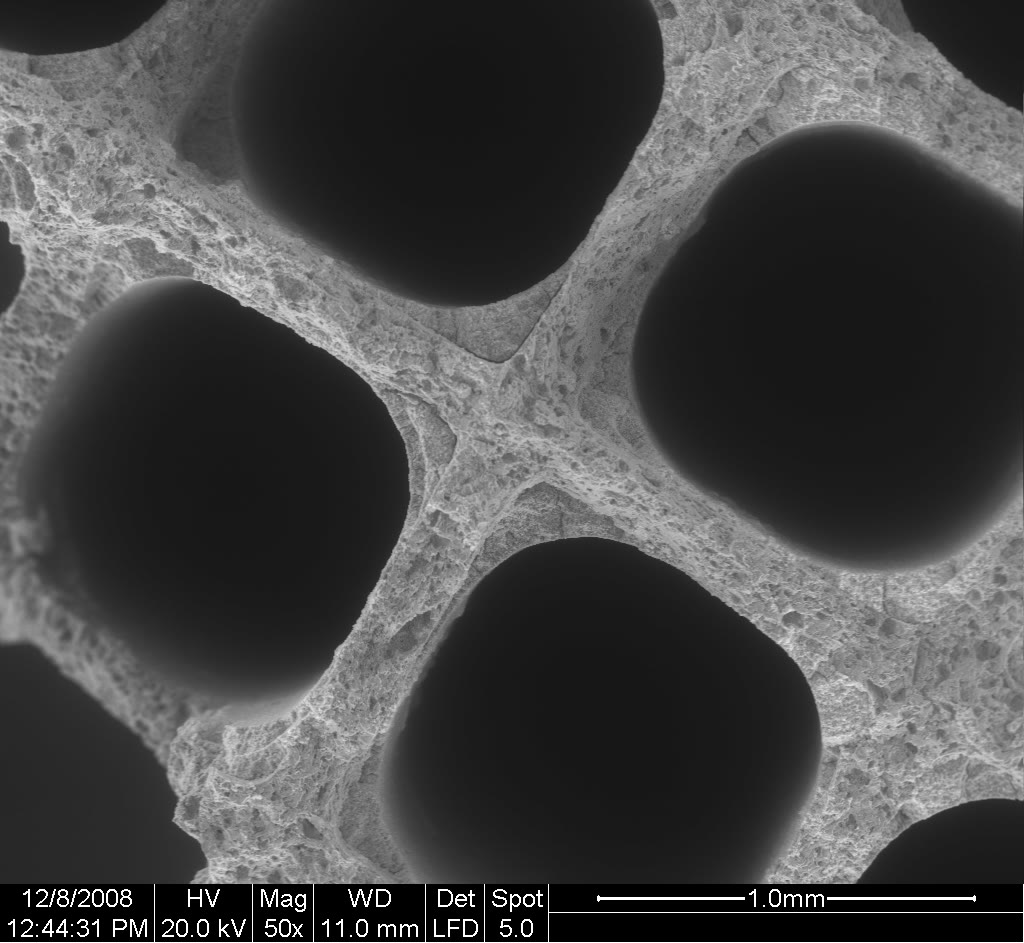
\includegraphics[width=0.48\linewidth]{images/book4/converter-sem.jpg}

{\small El panal cerámico de un convertidor catalítico visto con un microscopio electrónico
de barrido (barra de escala de \qty{1.0}{mm}): canales cuadrados separados por finas
paredes porosas, que llevan el recubrimiento de óxido y sus partículas metálicas.}
\end{omfigure}

\section{Adsorción}

\begin{definition}[Adsorción]\label{def:b3:surfaces-catalysis:adsorption}
La \emph{adsorción}\index{adsorcion@adsorción} es la acumulación de moléculas de un gas o de
un soluto en la superficie de un sólido o de un líquido. La molécula que se adsorbe es el
\emph{adsorbato}\index{adsorbato}, y el sólido, el \emph{adsorbente}\index{adsorbente};
el proceso inverso es la \emph{desorción}\index{desorcion@desorción}.
\end{definition}

\begin{definition}[Fisisorción, quimisorción]\label{def:b3:surfaces-catalysis:physi-chemi}
La \emph{fisisorción}\index{fisisorcion@fisisorción} es la \omterm{def:b3:surfaces-catalysis:adsorption}{adsorción} por fuerzas de van der Waals,
con entalpías de \omterm{def:b3:surfaces-catalysis:adsorption}{adsorción} de unas decenas de kilojulios por mol como mucho,
comparables a las entalpías de condensación, y sin cambio de la molécula.
La \emph{quimisorción}\index{quimisorcion@quimisorción} forma enlaces químicos con la superficie,
con entalpías de unos 40 a varios cientos de kilojulios por mol; puede
romper la molécula (quimisorción disociativa) y se detiene en una sola capa.
\end{definition}

\begin{omfigure}
\begin{tikzpicture}[font=\small, >=Stealth, x=1cm, y=1cm]
  \draw[->] (0,-2.6) -- (0,1.8) node[anchor=south] {energía};
  \draw[->] (0,0) -- (8.0,0) node[anchor=south east] {distancia a la superficie};
  \draw[omDef, thick] plot[smooth, tension=0.7] coordinates {(1.6,1.6) (2.2,-0.25) (2.8,-0.62) (3.6,-0.35) (5.0,-0.08) (7.5,0)};
  \draw[omThm, thick] plot[smooth, tension=0.6] coordinates {(0.45,1.6) (0.8,-1.2) (1.2,-2.2) (1.7,-1.6) (2.35,-0.15) (2.9,0.9) (3.5,1.5)};
  \node[omDef, anchor=north west, font=\scriptsize] at (3.4,-0.4) {\ce{H2} fisisorbido (precursor)};
  \node[omThm, anchor=west, font=\scriptsize] at (1.75,-1.9) {2 H quimisorbidos};
  \node[omThm, anchor=west, font=\scriptsize, align=left] at (3.55,1.45) {hacia $\mathrm{H} + \mathrm{H}$\\ lejos de la superficie};
  \fill (2.3,-0.2) circle (1.5pt);
  \node[font=\scriptsize] (cr) at (1.25,0.55) {cruce};
  \draw[black!60] (cr.south east) -- (2.27,-0.15);
\end{tikzpicture}

{\small Energía potencial de una molécula de hidrógeno que se acerca a una superficie metálica
(esquema). La molécula cae primero en el pozo poco profundo de la \omterm{def:b3:surfaces-catalysis:physi-chemi}{fisisorción};
donde esta curva corta la curva de dos átomos de H enlazados por separado, puede
disociarse hacia el pozo profundo de la \omterm{def:b3:surfaces-catalysis:physi-chemi}{quimisorción}. Si el cruce está por encima de cero,
la \omterm{def:b3:surfaces-catalysis:physi-chemi}{quimisorción} disociativa es activada.}
\end{omfigure}

Las superficies de las partículas metálicas exponen sobre todo las caras más densas de la red
FCC, (111) y (100). Sobre ellas, un \omterm{def:b3:surfaces-catalysis:adsorption}{adsorbato} puede situarse encima de un átomo
(sitio superior), entre dos (sitio puente) o en un hueco entre tres o cuatro, y la
energía de enlace varía de un sitio a otro.

\begin{omfigure}
\begin{tikzpicture}[font=\scriptsize]
  % fcc(111): hexagonal layer, spacing 0.6 cm
  \foreach \i in {0,...,5}{\foreach \j in {0,...,4}{
    \shade[ball color=black!25] ({0.6*\i+0.3*\j},{0.52*\j}) circle (0.29);}}
  \fill[omThm] (1.2+0.3*1,0.52) circle (0.07);
  \fill[omDef] ({0.6*2+0.3*2+0.3},{0.52*2}) circle (0.07);
  \fill[black] ({0.6*3+0.3*2+0.3},{0.52*2+0.17}) circle (0.07);
  \fill[black!60!green] ({0.6*1+0.3*3+0.3},{0.52*3-0.17}) circle (0.07);
  \node[anchor=north] at (2.1,-0.45) {fcc(111)};
  % fcc(100): square layer
  \begin{scope}[xshift=5.6cm]
  \foreach \i in {0,...,4}{\foreach \j in {0,...,4}{
    \shade[ball color=black!25] ({0.6*\i},{0.6*\j}) circle (0.29);}}
  \fill[omThm] (1.2,1.2) circle (0.07);
  \fill[omDef] (1.5,1.8) circle (0.07);
  \fill[black] (2.1,0.9) circle (0.07);
  \node[anchor=north] at (1.2,-0.45) {fcc(100)};
  \end{scope}
  \node[anchor=west, align=left] at (9.0,1.6) {\textcolor{omThm}{$\bullet$} superior\\ \textcolor{omDef}{$\bullet$} puente\\
    $\bullet$ hueco (de 3 o 4)\\ \textcolor{black!60!green}{$\bullet$} segundo hueco de 3 (111)};
\end{tikzpicture}

{\small Vistas desde arriba de las dos caras más densas de un metal cúbico centrado en las caras, con
los sitios de \omterm{def:b3:surfaces-catalysis:adsorption}{adsorción}: encima de un átomo, en puente entre dos y en los huecos entre
tres átomos en (111) (de dos tipos, sobre un átomo de la segunda capa o no) o
cuatro átomos en (100).}
\end{omfigure}

\begin{definition}[Grado de recubrimiento, monocapa]\label{def:b3:surfaces-catalysis:coverage}
El \emph{grado de recubrimiento}\index{grado de recubrimiento} $\theta$ de una superficie es la
fracción de sus sitios de \omterm{def:b3:surfaces-catalysis:adsorption}{adsorción} que están ocupados. Una
\emph{monocapa}\index{monocapa} es una sola capa completa de \omterm{def:b3:surfaces-catalysis:adsorption}{adsorbato}, $\theta = 1$.
\end{definition}

\section{Isotermas}

\begin{theorem}[Isoterma de Langmuir]\label{thm:b3:surfaces-catalysis:langmuir}
Si una superficie tiene sitios idénticos e independientes, cada uno capaz de retener una molécula, el
\omterm{def:b3:surfaces-catalysis:coverage}{grado de recubrimiento} en equilibrio con un gas a la presión $p$ es
\[
  \theta = \frac{Kp}{1 + Kp},
\]
donde $K$, la constante de equilibrio de \omterm{def:b3:surfaces-catalysis:adsorption}{adsorción}, solo depende de la
temperatura. Es la \emph{isoterma de Langmuir}\index{isoterma de Langmuir}.
\end{theorem}

\begin{proof}
Demostración cinética. Las moléculas se adsorben en los sitios libres a la velocidad $k_ap(1 - \theta)N$ ($N$
sitios) y se desorben a la velocidad $k_d\theta N$. En el equilibrio ambas son iguales: $\theta/(1 - \theta)
= (k_a/k_d)p$, que se reordena en el resultado con $K = k_a/k_d$.

Demostración estadística. $M$ moléculas sobre $N$ sitios pueden disponerse de $N!/(M!(N - M)!)$ maneras,
y cada molécula adsorbida tiene una función de partición interna $q_{\mathrm s}$ (sus
vibraciones contra la superficie y su energía de enlace). Con la fórmula de Stirling,
el potencial químico de las moléculas adsorbidas es $\mu_{\mathrm s} = -kT\ln\bigl(q_{\mathrm s}\frac{1 - \theta}{\theta}\bigr)$;
el del gas ideal es $\mu_{\mathrm g} = \mu_{\mathrm g}^\circ + kT\ln(p/p^\circ)$. El equilibrio, $\mu_{\mathrm s} = \mu_{\mathrm g}$, da
$\theta/(1 - \theta) = q_{\mathrm s}\eu^{\mu_{\mathrm g}^\circ/kT}p/p^\circ$: la misma ley, con $K$ expresada en términos de
funciones de partición.
\end{proof}

A baja presión, $\theta \approx Kp$ (régimen de Henry); a alta presión, $\theta \to 1$. El
\omterm{def:b3:surfaces-catalysis:coverage}{grado de recubrimiento} vale un medio en $p = 1/K$.

\begin{proposition}[Adsorción disociativa]\label{prop:b3:surfaces-catalysis:dissociative}
Para un gas diatómico que se disocia sobre dos sitios, $\mathrm{H_2} + 2\,{*} \to 2\,\mathrm{H}{*}$ (${*}$: un sitio libre),
\[
  \theta = \frac{(Kp)^{1/2}}{1 + (Kp)^{1/2}},
\]
de modo que $\theta \propto \sqrt p$ a baja presión.
\end{proposition}

\begin{proof}
La \omterm{def:b3:surfaces-catalysis:adsorption}{adsorción} necesita dos sitios libres, a la velocidad $k_ap(1 - \theta)^2$; la \omterm{def:b3:surfaces-catalysis:adsorption}{desorción} necesita que dos
átomos adsorbidos se recombinen, a la velocidad $k_d\theta^2$. La igualdad da $\theta/(1 - \theta) =
(Kp)^{1/2}$.
\end{proof}

\begin{proposition}[Adsorción competitiva]\label{prop:b3:surfaces-catalysis:competitive}
Dos gases A y B que compiten por los mismos sitios los recubren con
\[
  \theta_{\mathrm A} = \frac{K_{\mathrm A}p_{\mathrm A}}{1 + K_{\mathrm A}p_{\mathrm A} + K_{\mathrm B}p_{\mathrm B}}, \qquad
  \theta_{\mathrm B} = \frac{K_{\mathrm B}p_{\mathrm B}}{1 + K_{\mathrm A}p_{\mathrm A} + K_{\mathrm B}p_{\mathrm B}} .
\]
\end{proposition}

\begin{proof}
Para cada gas, $k_{a,\mathrm A}p_{\mathrm A}(1 - \theta_{\mathrm A} - \theta_{\mathrm B}) = k_{d,\mathrm A}\theta_{\mathrm A}$, y lo mismo para B. Por tanto,
$\theta_{\mathrm A} = K_{\mathrm A}p_{\mathrm A}\theta_\ast$ y $\theta_{\mathrm B} = K_{\mathrm B}p_{\mathrm B}\theta_\ast$, con $\theta_\ast = 1 - \theta_{\mathrm A} - \theta_{\mathrm B}$ la fracción libre; sumando,
$1 - \theta_\ast = \theta_\ast(K_{\mathrm A}p_{\mathrm A} + K_{\mathrm B}p_{\mathrm B})$.
\end{proof}

\begin{definition}[Entalpía isostérica de adsorción]\label{def:b3:surfaces-catalysis:isosteric}
La \emph{entalpía isostérica de adsorción}\index{entalpia isosterica de adsorcion@entalpía isostérica de adsorción}
$\Delta_{\mathrm{ads}}H$ es la entalpía molar de \omterm{def:b3:surfaces-catalysis:adsorption}{adsorción} a \omterm{def:b3:surfaces-catalysis:coverage}{grado de recubrimiento} fijo,
obtenida a partir de las presiones que dan el mismo \omterm{def:b3:surfaces-catalysis:coverage}{grado de recubrimiento} a distintas
temperaturas.
\end{definition}

\begin{proposition}[Entalpía isostérica]\label{prop:b3:surfaces-catalysis:isosteric}
A \omterm{def:b3:surfaces-catalysis:coverage}{grado de recubrimiento} constante,
\[
  \Bigl(\frac{\partial\ln p}{\partial T}\Bigr)_\theta = -\frac{\Delta_{\mathrm{ads}}H}{RT^2} .
\]
\end{proposition}

\begin{proof}
A $\theta$ constante, $Kp$ es constante (para una superficie de Langmuir; en general, el mismo
razonamiento vale con la constante de equilibrio a ese \omterm{def:b3:surfaces-catalysis:coverage}{grado de recubrimiento}), luego $\ln p =
\text{cte} - \ln K$. Por la ecuación de van 't Hoff, $\dd\ln K/\dd T = \Delta_{\mathrm{ads}}H/RT^2$ (con $K$
referida a una presión estándar).
\end{proof}

Como la \omterm{def:b3:surfaces-catalysis:adsorption}{adsorción} es exotérmica, las temperaturas más altas necesitan presiones más altas para
el mismo \omterm{def:b3:surfaces-catalysis:coverage}{grado de recubrimiento}: las isotermas de la figura bajan cuando $T$ sube.

\begin{theorem}[Isoterma BET]\label{thm:b3:surfaces-catalysis:bet}
Si las moléculas se adsorben en capas sucesivas, la primera con una constante de enlace
característica de la superficie y las demás con el equilibrio de condensación
del líquido, la cantidad adsorbida a la presión relativa $x = p/p^*$ ($p^*$: presión de vapor
del \omterm{def:b3:surfaces-catalysis:adsorption}{adsorbato} líquido) es
\[
  \frac{v}{v_{\mathrm m}} = \frac{cx}{(1 - x)(1 - x + cx)},
\]
donde $v_{\mathrm m}$ es la cantidad correspondiente a una \omterm{def:b3:surfaces-catalysis:coverage}{monocapa} y $c$ una constante relacionada con la
diferencia entre las entalpías de \omterm{def:b3:surfaces-catalysis:adsorption}{adsorción} en la primera capa y de
condensación. Es la \emph{isoterma BET}\index{isoterma BET} (Brunauer,
Emmett y Teller).
\end{theorem}

\begin{proof}
Sea $s_i$ la fracción de la superficie cubierta exactamente por $i$ capas. El
balance de cada capa, como en la demostración de Langmuir, da $s_1 = cxs_0$ y $s_i =
xs_{i-1}$ para $i \ge 2$, luego $s_i = cx^is_0$. La cantidad adsorbida es $v/v_{\mathrm m} =
\sum_iis_i/\sum_is_i$. Con $\sum_{i\ge1}x^i = x/(1 - x)$ y $\sum_{i\ge1}ix^i = x/(1 - x)^2$:
\[
  \frac{v}{v_{\mathrm m}} = \frac{cs_0\,x/(1 - x)^2}{s_0[1 + cx/(1 - x)]} = \frac{cx}{(1 - x)(1 - x + cx)} .
\]
\end{proof}

Reordenada, $\dfrac{x}{v(1 - x)} = \dfrac{1}{v_{\mathrm m}c} + \dfrac{c - 1}{v_{\mathrm m}c}\,x$: una recta cuya pendiente y
ordenada en el origen dan $v_{\mathrm m}$ y $c$, normalmente válida para $0.05 < x < 0.30$.

\begin{definition}[Superficie específica]\label{def:b3:surfaces-catalysis:surface-area}
La \emph{superficie específica}\index{superficie especifica@superficie específica} de un sólido es su
área superficial por unidad de masa, incluidas las paredes de sus poros.
\end{definition}

\begin{method}[Superficie específica a partir de una isoterma de nitrógeno]\label{met:b3:surfaces-catalysis:bet-area}
\begin{enumerate}
  \item Desgasificar la muestra a vacío calentándola; enfriarla en nitrógeno líquido
        (\qty{77}{K}).
  \item Medir el volumen de nitrógeno adsorbido (reducido a condiciones normales)
        a presiones relativas entre 0.05 y 0.30.
  \item Representar $x/(v(1 - x))$ en función de $x$; a partir de la pendiente y la ordenada en el origen,
        $v_{\mathrm m} = 1/(\text{pendiente} + \text{ordenada})$ y $c = 1 + \text{pendiente}/\text{ordenada}$.
  \item Área $= n_{\mathrm m}N_Aa_{\mathrm m}$, con $n_{\mathrm m}$ la cantidad en la \omterm{def:b3:surfaces-catalysis:coverage}{monocapa} y $a_{\mathrm m} = \qty{0.162}{nm^2}$
        el área convencional de una molécula de nitrógeno adsorbida.
\end{enumerate}
\end{method}

\begin{omfigure}
\begin{tikzpicture}
\begin{axis}[name=la, width=0.31\linewidth, height=5.0cm, xmin=0, xmax=100, ymin=0, ymax=1.05,
  axis lines=left, xlabel={$p$ / kPa}, ylabel={$\theta$}, tick label style={font=\small},
  label style={font=\small}, title={\small Langmuir}]
\addplot[omDef, thick] table[x=p_kPa, y=T300] {figdata/out/bachelor-3-langmuir-bet-langmuir.dat};
\addplot[omThm, thick] table[x=p_kPa, y=T350] {figdata/out/bachelor-3-langmuir-bet-langmuir.dat};
\node[font=\scriptsize, omDef, anchor=south east] at (axis cs:98,0.92) {\qty{300}{K}};
\node[font=\scriptsize, omThm, anchor=north east] at (axis cs:98,0.45) {\qty{350}{K}};
\end{axis}
\begin{axis}[name=be, at={(la.east)}, anchor=west, xshift=1.9cm, width=0.31\linewidth, height=5.0cm,
  xmin=0, xmax=0.9, ymin=0, ymax=200, axis lines=left, xlabel={$p/p^*$},
  ylabel={$v$ / \unit{cm^3.g^{-1}}}, tick label style={font=\small}, label style={font=\small},
  title={\small BET}]
\addplot[black, thick] table[x=x, y=v] {figdata/out/bachelor-3-langmuir-bet-bet.dat};
\addplot[only marks, mark=*, mark size=1.4pt, omDef] table[x=x, y=v] {figdata/out/bachelor-3-langmuir-bet-data.dat};
\draw[black!40, dashed] (axis cs:0,45) -- (axis cs:0.9,45);
\node[font=\scriptsize, anchor=south east] at (axis cs:0.88,45) {$v_{\mathrm m}$};
\end{axis}
\begin{axis}[at={(be.east)}, anchor=west, xshift=2.1cm, width=0.31\linewidth, height=5.0cm,
  xmin=0, xmax=0.35, ymin=0, ymax=0.0085, axis lines=left, xlabel={$x = p/p^*$},
  ylabel={$x/(v(1 - x))$}, tick label style={font=\small}, label style={font=\small},
  scaled y ticks=false, yticklabel style={/pgf/number format/fixed, /pgf/number format/precision=3},
  title={\small gráfica BET}]
\addplot[black, thin] table[x=x, y=y] {figdata/out/bachelor-3-langmuir-bet-line.dat};
\addplot[only marks, mark=*, mark size=1.4pt, omDef] table[x=x, y=y] {figdata/out/bachelor-3-langmuir-bet-data.dat};
\end{axis}
\end{tikzpicture}

{\small Izquierda: \omterm{thm:b3:surfaces-catalysis:langmuir}{isotermas de Langmuir} de una \omterm{def:b3:surfaces-catalysis:physi-chemi}{quimisorción} modelo ($\Delta_{\mathrm{ads}}H = \qty{-40}{kJ/mol}$) a
dos temperaturas. Centro: una \omterm{thm:b3:surfaces-catalysis:bet}{isoterma BET} (modelo, $v_{\mathrm m} = \qty{45}{cm^3.g^{-1}}$, $c = 120$), con los
puntos del problema de fin de semana; las capas se apilan y la cantidad diverge cerca de
$p = p^*$, donde el gas condensa. Derecha: la gráfica BET lineal de los mismos puntos.}
\end{omfigure}

\section{Cinética de las reacciones superficiales}

\begin{definition}[Mecanismos de Langmuir--Hinshelwood y de Eley--Rideal]\label{def:b3:surfaces-catalysis:mechanisms}
En el \emph{mecanismo de Langmuir--Hinshelwood}\index{mecanismo de Langmuir--Hinshelwood}
ambos reactivos están adsorbidos y reaccionan sobre la superficie; en el
\emph{mecanismo de Eley--Rideal}\index{mecanismo de Eley--Rideal}, un reactivo adsorbido
reacciona con una molécula que llega desde el gas.
\end{definition}

\begin{proposition}[Velocidad de Langmuir--Hinshelwood]\label{prop:b3:surfaces-catalysis:lh-rate}
Si los equilibrios de \omterm{def:b3:surfaces-catalysis:adsorption}{adsorción} son rápidos y la reacción superficial de A y B adsorbidos
es la etapa determinante,
\[
  r = k\theta_{\mathrm A}\theta_{\mathrm B} = \frac{kK_{\mathrm A}p_{\mathrm A}K_{\mathrm B}p_{\mathrm B}}{(1 + K_{\mathrm A}p_{\mathrm A} + K_{\mathrm B}p_{\mathrm B})^2},
\]
que, a $p_{\mathrm B}$ fija, es máxima cuando $K_{\mathrm A}p_{\mathrm A} = 1 + K_{\mathrm B}p_{\mathrm B}$ y disminuye después a medida que A expulsa a B de la
superficie.
\end{proposition}

\begin{proof}
Los \omterm{def:b3:surfaces-catalysis:coverage}{grados de recubrimiento} son los de la \cref{prop:b3:surfaces-catalysis:competitive}. Con $u =
K_{\mathrm A}p_{\mathrm A}$ y $a = 1 + K_{\mathrm B}p_{\mathrm B}$, $r \propto u/(a + u)^2$, cuya derivada, $(a - u)/(a + u)^3$, se anula en
$u = a$.
\end{proof}

\begin{proposition}[Velocidad de Eley--Rideal]\label{prop:b3:surfaces-catalysis:er-rate}
Si A adsorbido reacciona con B gaseoso,
\[
  r = k\theta_{\mathrm A}p_{\mathrm B} = \frac{kK_{\mathrm A}p_{\mathrm A}p_{\mathrm B}}{1 + K_{\mathrm A}p_{\mathrm A}},
\]
que crece con $p_{\mathrm A}$ hasta una meseta, sin máximo.
\end{proposition}

\begin{proof}
B no compite por los sitios: $\theta_{\mathrm A}$ es el \omterm{def:b3:surfaces-catalysis:coverage}{grado de recubrimiento} de Langmuir de A solo, y la
velocidad es proporcional a él y a la frecuencia de colisión de B con la superficie,
proporcional a $p_{\mathrm B}$.
\end{proof}

\begin{method}[LH o ER a partir de la dependencia con la presión]\label{met:b3:surfaces-catalysis:mechanism-from-rate}
\begin{enumerate}
  \item Medir la velocidad en función de la presión de cada reactivo, manteniendo fija la
        del otro.
  \item Un máximo seguido de un descenso (orden negativo a alta presión):
        Langmuir--Hinshelwood, pues el reactivo inhibe al ocupar los sitios.
  \item Un aumento hasta una meseta en un reactivo y primer orden en el otro a todas las
        presiones: Eley--Rideal.
  \item Confirmar con marcaje isotópico o espectroscopia de superficie; la mayoría de las reacciones
        catalíticas resultan ser del tipo Langmuir--Hinshelwood.
\end{enumerate}
\end{method}

\begin{omfigure}
\begin{tikzpicture}
\begin{axis}[width=0.6\linewidth, height=5.4cm, xmin=0, xmax=10, ymin=0, ymax=0.3,
  axis lines=left, xlabel={$p_{\mathrm A}$ (reducida)}, ylabel={velocidad (reducida)},
  tick label style={font=\small}, label style={font=\small},
  legend style={font=\scriptsize, draw=none, at={(1.03,0.98)}, anchor=north west}, legend cell align=left]
\addplot[omDef!50, thick] table[x=pA, y=pB05] {figdata/out/bachelor-3-surface-rates.dat};
\addplot[omDef, thick] table[x=pA, y=pB1] {figdata/out/bachelor-3-surface-rates.dat};
\addplot[black, thick] table[x=pA, y=pB3] {figdata/out/bachelor-3-surface-rates.dat};
\addplot[omThm, thick, dashed] table[x=pA, y=ER] {figdata/out/bachelor-3-surface-rates.dat};
\legend{{LH, $p_{\mathrm B} = 0.5$}, {LH, $p_{\mathrm B} = 1$}, {LH, $p_{\mathrm B} = 3$}, {ER ($\times\frac14$)}}
\end{axis}
\end{tikzpicture}

{\small Velocidades de una reacción superficial bimolecular en función de la presión de A
(unidades reducidas, $K_{\mathrm A} = K_{\mathrm B} = 1$). Langmuir--Hinshelwood: cada curva tiene su máximo en $K_{\mathrm A}p_{\mathrm A} =
1 + K_{\mathrm B}p_{\mathrm B}$ y disminuye después a medida que A desplaza a B. Eley--Rideal (trazo discontinuo, escalada): una meseta.}
\end{omfigure}

\begin{proposition}[Energía de activación aparente]\label{prop:b3:surfaces-catalysis:apparent-ea}
Para una reacción superficial unimolecular con \omterm{def:b3:surfaces-catalysis:adsorption}{adsorción} de Langmuir, $r = k\theta = kKp/(1 + Kp)$.
A bajo \omterm{def:b3:surfaces-catalysis:coverage}{grado de recubrimiento}, la energía de activación medida es $E_{a,\mathrm{app}} = E_a + \Delta_{\mathrm{ads}}H$; a
alto \omterm{def:b3:surfaces-catalysis:coverage}{grado de recubrimiento} es $E_a$.
\end{proposition}

\begin{proof}
A bajo \omterm{def:b3:surfaces-catalysis:coverage}{grado de recubrimiento}, $r \approx kKp$, luego $\dd\ln r/\dd T = \dd\ln k/\dd T + \dd\ln K/\dd T = (E_a + \Delta_{\mathrm{ads}}H)/RT^2$.
A alto \omterm{def:b3:surfaces-catalysis:coverage}{grado de recubrimiento}, $\theta \approx 1$ y $r \approx k$.
\end{proof}

Como $\Delta_{\mathrm{ads}}H < 0$, una reacción sobre una superficie poco cubierta parece más fácil de lo que indica su
barrera real: subir la temperatura acelera la etapa superficial pero vacía
la superficie.

\begin{definition}[Principio de Sabatier, curva en volcán]\label{def:b3:surfaces-catalysis:sabatier}
El \emph{principio de Sabatier}\index{principio de Sabatier} afirma que el mejor
catalizador no enlaza los reactivos ni demasiado débilmente (no se adsorben ni se
activan) ni demasiado fuertemente (los productos no se van y bloquean los sitios). Una
\emph{curva en volcán}\index{curva en volcan@curva en volcán} de la actividad de una serie de
catalizadores en función de una energía de enlace tiene un máximo a enlace intermedio.
\end{definition}

\begin{omfigure}
\begin{tikzpicture}[font=\small, >=Stealth]
  \draw[->] (0,0) -- (7.2,0) node[anchor=north east] {fuerza de enlace del adsorbato};
  \draw[->] (0,0) -- (0,3.6) node[anchor=south] {actividad};
  \draw[omDef, very thick] (0.4,0.3) -- (3.4,3.0) -- (6.6,0.4);
  \node[anchor=south, align=center, font=\scriptsize] at (1.35,2.0) {enlace muy débil:\\ reactivos no\\ activados};
  \node[anchor=south, align=center, font=\scriptsize] at (5.9,2.0) {enlace muy fuerte:\\ los productos\\ bloquean los sitios};
  \node[anchor=south, font=\scriptsize] at (3.4,3.05) {mejor catalizador};
\end{tikzpicture}

{\small Una \omterm{def:b3:surfaces-catalysis:sabatier}{curva en volcán} (cualitativa): la actividad de una serie de catalizadores
en función de la fuerza con la que enlazan un intermedio clave.}
\end{omfigure}

\section{Catalizadores industriales}

\begin{definition}[Diseño de catalizadores]\label{def:b3:surfaces-catalysis:catalyst-design}
Un \emph{soporte de catalizador}\index{soporte de catalizador} es un sólido poroso de gran área
(alúmina, sílice, carbono) que lleva pequeñas partículas de la fase activa. Un
\emph{promotor}\index{promotor} es un aditivo, inactivo por sí solo, que aumenta la
actividad, la selectividad o la estabilidad. Un \emph{veneno de catalizador}\index{veneno de catalizador}
es una sustancia que se une fuertemente a los \omterm{def:b3:complex-kinetics:enzyme}{sitios activos} y los bloquea.
La \emph{dispersión metálica}\index{dispersion metalica@dispersión metálica} $D$ es la fracción de los átomos del metal
que están en la superficie. La \emph{sinterización}\index{sinterizacion@sinterización} es el crecimiento de
las partículas a alta temperatura, que reduce la dispersión.
\end{definition}

\begin{method}[Dispersión y tamaño de partícula a partir de la quimisorción de hidrógeno]\label{met:b3:surfaces-catalysis:dispersion}
\begin{enumerate}
  \item Reducir el catalizador en hidrógeno, hacer vacío y medir el volumen de \ce{H2}
        quimisorbido (reducido a condiciones normales) sobre el metal; el
        soporte no adsorbe nada.
  \item Suponer un átomo de H por átomo metálico superficial: $D = n_{\ce{H}}/n_{\text{metal}}$.
  \item Para esferas de diámetro $d$, $D = 6(v_{\mathrm{at}}/a_{\mathrm{at}})/d$, con $v_{\mathrm{at}}$ el volumen por átomo en el
        seno del metal y $a_{\mathrm{at}}$ el área por átomo superficial; por tanto, $d = 6v_{\mathrm{at}}/(a_{\mathrm{at}}D)$.
\end{enumerate}
\end{method}

La síntesis del amoniaco, $\ce{N2 + 3 H2 <=> 2 NH3}$, opera a unos 400 a \qty{500}{\celsius} y de 100 a
\qty{300}{bar} sobre hierro promovido con óxido de potasio y alúmina: la alúmina impide que
los cristalitos de hierro se sintericen y el potasio aumenta la actividad. La
etapa determinante es la \omterm{def:b3:surfaces-catalysis:physi-chemi}{quimisorción} disociativa del \ce{N2}, cuyo triple
enlace es el más difícil de romper. Así se fijan unos 150 millones de toneladas de nitrógeno al
año.
% ledger: nh3:world-2024
La oxidación de \ce{SO2} a \ce{SO3}, sobre óxido de vanadio(V) promovido
con sulfato de potasio, es la etapa clave de la fabricación del ácido sulfúrico.

El convertidor de tres vías de los motores de gasolina oxida el CO y los hidrocarburos y
reduce los óxidos de nitrógeno al mismo tiempo, sobre platino y paladio (oxidación)
y rodio (reducción del NO), dispersos sobre alúmina con óxido de cerio, que
almacena y libera oxígeno. Solo funciona en una estrecha ventana en torno a la
relación aire--combustible estequiométrica: con exceso de aire el NO no se reduce, y con
exceso de combustible el CO no se oxida; un sensor de oxígeno en el escape mantiene el
motor en esa ventana. El plomo de la gasolina con plomo envenena el metal, que es una de las
razones por las que desapareció la gasolina con plomo. Las zeolitas, aluminosilicatos cristalinos con
poros de tamaño molecular y sitios ácidos, craquean las moléculas grandes de las fracciones pesadas del
petróleo para dar gasolina y solo admiten las moléculas que caben en sus canales.

\begin{omfigure}
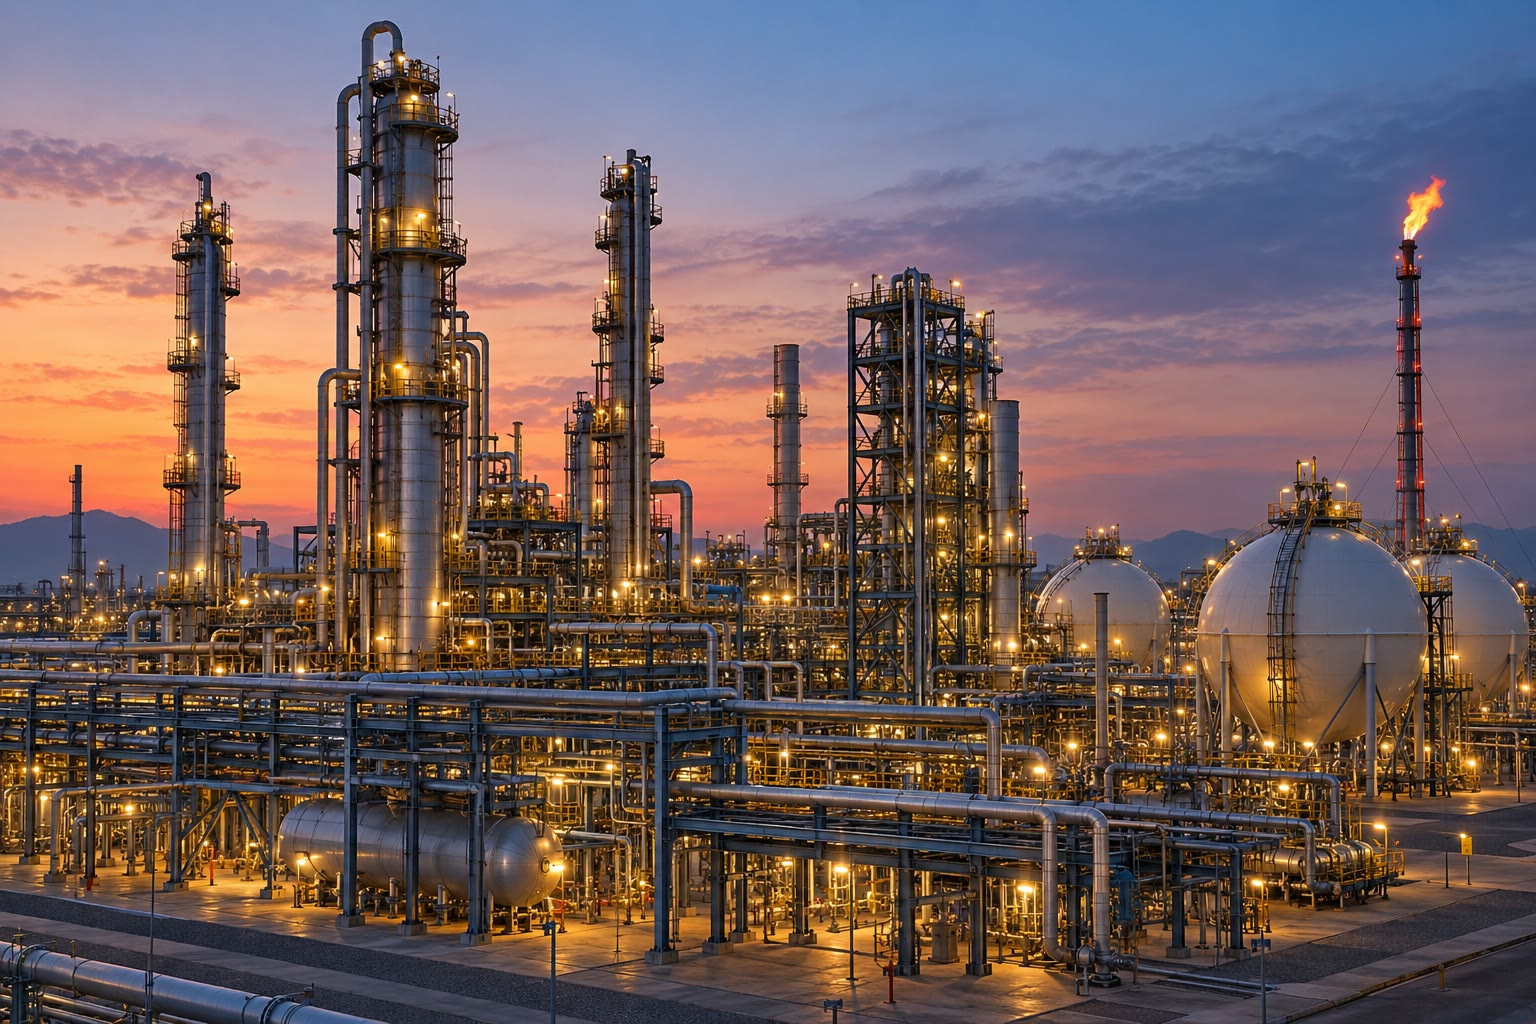
\includegraphics[width=0.6\linewidth]{images/book4/ai/b3-16-ammonia-plant.jpg}

{\small Una planta de síntesis de amoniaco. El reactor, su corazón, contiene toneladas de
catalizador de hierro promovido; la mayor parte de la planta prepara el hidrógeno y recicla
el gas no convertido.}
\end{omfigure}

\section{Observar las superficies}

\begin{definition}[Espectroscopia de desorción térmica]\label{def:b3:surfaces-catalysis:tpd}
La \emph{espectroscopia de desorción térmica}\index{espectroscopia de desorcion termica@espectroscopia de desorción térmica}
calienta a velocidad constante una superficie que lleva un \omterm{def:b3:surfaces-catalysis:adsorption}{adsorbato} y registra el
gas que se desorbe con un espectrómetro de masas; cada estado de enlace da un pico, cuya
temperatura aumenta con su energía de activación de \omterm{def:b3:surfaces-catalysis:adsorption}{desorción}.
\end{definition}

La posición de un pico de \omterm{def:b3:surfaces-catalysis:adsorption}{desorción} da la energía de \omterm{def:b3:surfaces-catalysis:adsorption}{desorción} (para una \omterm{def:b3:surfaces-catalysis:adsorption}{desorción} de primer orden,
$E_d \approx RT_{\mathrm p}[\ln(\nu T_{\mathrm p}/\beta) - 3.64]$, con $\beta$ la velocidad de calentamiento y $\nu \approx \qty{e13}{s^{-1}}$,
que se admite), y su área, la cantidad adsorbida. La espectroscopia fotoelectrónica de
rayos X (XPS) mide las energías de enlace de los electrones internos de los átomos superficiales,
que identifican los elementos y sus estados de oxidación en los primeros
nanómetros. El microscopio de \omterm{def:b3:quantum-model-systems:tunnelling}{efecto túnel} desplaza una punta afilada a unas décimas
de nanómetro por encima de una superficie conductora; la corriente túnel
(\cref{ch:b3:quantum-model-systems}) disminuye alrededor de un orden de magnitud por
cada \qty{0.1}{nm} de distancia adicional, de modo que mantenerla constante durante el barrido
cartografía la superficie átomo a átomo.

\begin{inthelab}[Una medida BET]
Se pesan unos \qty{0.2}{g} de muestra en un tubo de vidrio con un bulbo, se desgasifican
durante horas a vacío a 150 a \qty{300}{\celsius}, se pesan de nuevo y se montan en el
instrumento, con el bulbo sumergido en un dewar de nitrógeno líquido. El instrumento
admite nitrógeno en pequeñas dosis y mide la presión de equilibrio tras cada una,
deduciendo la cantidad adsorbida a partir del balance del gas; el volumen muerto del tubo
se mide con helio, que no se adsorbe.
\end{inthelab}

\begin{safety}{\ghs[0.7cm]{GHS06}\ghs[0.7cm]{GHS07}\ghs[0.7cm]{GHS08}\ghs[0.7cm]{GHS09}}
% ledger: ghs4:V2O5, ghs4:Ni
Los catalizadores metálicos reducidos (níquel, paladio o platino finamente divididos sobre un
soporte, recién reducidos en hidrógeno) pueden inflamarse en contacto con el aire: se
manipulan bajo gas inerte y se pasivan antes de almacenarlos. El níquel es un sensibilizante
cutáneo y un posible cancerígeno; el óxido de vanadio(V) es tóxico por inhalación
e ingestión y puede provocar cáncer. Los catalizadores en polvo se pesan en un recinto
ventilado.
\end{safety}

\begin{history}[Langmuir y el catalizador del amoniaco]
Irving Langmuir, que trabajaba en bombillas en un laboratorio industrial, dedujo
su isoterma en 1916--1918 a partir de la idea de que los gases adsorbidos forman una capa de una
molécula de espesor, y recibió el premio Nobel de Química de 1932 por su química de
superficies. Unos años antes, Alwin Mittasch había organizado la búsqueda de un
catalizador práctico para el amoniaco: se ensayaron miles de composiciones en pequeños
reactores de alta presión antes de elegir el catalizador de hierro promovido, todavía en uso.
Fue uno de los primeros cribados sistemáticos de catalizadores.
\end{history}

\section{Ejercicios}

\begin{exercise}[$\star$]\label{exo:b3:surfaces-catalysis:1}
Un gas cubre el 40\,\% de una superficie de Langmuir a \qty{2.0}{kPa}. Calcúlense $K$ y el \omterm{def:b3:surfaces-catalysis:coverage}{grado de recubrimiento} a
\qty{10}{kPa}.
\end{exercise}

\begin{exercise}[$\star$]\label{exo:b3:surfaces-catalysis:2}
Se miden dos entalpías de \omterm{def:b3:surfaces-catalysis:adsorption}{adsorción} sobre un metal: $-20$ y \qty{-150}{kJ/mol}. ¿Cuál
es una \omterm{def:b3:surfaces-catalysis:physi-chemi}{fisisorción} y cuál una \omterm{def:b3:surfaces-catalysis:physi-chemi}{quimisorción}? ¿Cuál podría ser disociativa?
\end{exercise}

\begin{exercise}[$\star$]\label{exo:b3:surfaces-catalysis:3}
Cuéntense, por átomo superficial, los sitios superiores, puente y huecos de una cara (100) y de
una cara (111) de un metal FCC.
\end{exercise}

\begin{exercise}[$\star$]\label{exo:b3:surfaces-catalysis:4}
Un catalizador transforma \qty{3.0e-6}{mol} de reactivo por gramo y por segundo y lleva
\qty{1.5e-5}{mol} de sitios superficiales por gramo. Calcúlese la frecuencia de recambio.
\end{exercise}

\begin{exercise}[$\star\star$]\label{exo:b3:surfaces-catalysis:5}
El hidrógeno se adsorbe de forma disociativa con $\theta = 0.10$ a \qty{1.0}{kPa}. Calcúlese $\theta$ a \qty{4.0}{kPa}.
\end{exercise}

\begin{exercise}[$\star\star$]\label{exo:b3:surfaces-catalysis:6}
El CO ($K = \qty{10}{kPa^{-1}}$) y el \ce{O2} ($K = \qty{0.5}{kPa^{-1}}$, no disociativo en este modelo sencillo)
compiten por los sitios de una superficie de platino a 1.0 y \qty{5.0}{kPa}. Calcúlense los dos
\omterm{def:b3:surfaces-catalysis:coverage}{grados de recubrimiento} y coméntese la velocidad de oxidación del CO.
\end{exercise}

\begin{exercise}[$\star\star$]\label{exo:b3:surfaces-catalysis:7}
Un \omterm{def:b3:surfaces-catalysis:coverage}{grado de recubrimiento} alcanzado a \qty{1.0}{kPa} a \qty{300}{K} necesita \qty{8.0}{kPa} a \qty{350}{K}. Calcúlese la \omterm{def:b3:surfaces-catalysis:isosteric}{entalpía
isostérica de adsorción}.
\end{exercise}

\begin{exercise}[$\star\star$]\label{exo:b3:surfaces-catalysis:8}
% ledger: sa:N2.am, const:Vm1, const:NA
Un carbón activo tiene $v_{\mathrm m} = \qty{120}{cm^3.g^{-1}}$ (condiciones normales, 273.15 K y
\qty{101.325}{kPa}). Calcúlese su área BET.
\end{exercise}

\begin{exercise}[$\star\star$]\label{exo:b3:surfaces-catalysis:9}
La velocidad de $\ce{2 CO + O2 -> 2 CO2}$ sobre platino aumenta, pasa por un máximo y disminuye cuando $p(\ce{CO})$
aumenta a $p(\ce{O2})$ fija. ¿Qué mecanismo indica esto, y por qué inhibe el CO
la reacción?
\end{exercise}

\begin{exercise}[$\star\star\star$]\label{exo:b3:surfaces-catalysis:10}
Una reacción superficial tiene una energía de activación real de \qty{100}{kJ/mol}; el reactivo tiene
$\Delta_{\mathrm{ads}}H = \qty{-60}{kJ/mol}$. ¿Qué energía de activación se mide a bajo y a alto
\omterm{def:b3:surfaces-catalysis:coverage}{grado de recubrimiento}? Esbócese $\ln r$ en función de $1/T$ en un intervalo amplio.
\end{exercise}

\begin{exercise}[$\star\star\star$]\label{exo:b3:surfaces-catalysis:11}
El azufre se adsorbe sobre un catalizador de níquel con un \omterm{def:b3:surfaces-catalysis:coverage}{grado de recubrimiento} de 0.10 (átomos de azufre por
Ni superficial), y cada átomo de azufre bloquea cuatro sitios. ¿Qué fracción de la actividad
queda para una reacción que necesita un sitio libre? ¿Y dos sitios libres adyacentes (supónganse
sitios bloqueados situados al azar)?
\end{exercise}

\begin{exercise}[$\star\star\star$]\label{exo:b3:surfaces-catalysis:12}
Para la síntesis del amoniaco, tres metales enlazan el nitrógeno atómico con entalpías de
$-150$, $-250$ y \qty{-400}{kJ/mol} (datos del ejercicio). Según el \omterm{def:b3:surfaces-catalysis:sabatier}{principio de
Sabatier}, ¿cuál es probablemente el mejor catalizador, y qué limita a los otros dos?
\end{exercise}

\section{Problema: medir un catalizador}

\begin{problem}[{Problema de fin de semana --- medir un catalizador: el área BET de un
catalizador de platino soportado, su dispersión metálica y su tamaño de partícula a partir de la
quimisorción de hidrógeno, y la frecuencia de recambio de una hidrogenación}]
\label{pb:b3:surfaces-catalysis:1}
% ledger: sa:N2.am, lat:Pt, aw:Pt, const:Vm1, const:NA
Un catalizador contiene un 1.00\,\% en masa de platino sobre alúmina. Datos del problema:
isoterma de nitrógeno a \qty{77}{K} (volúmenes en condiciones normales, 273.15 K y
\qty{101.325}{kPa}, por gramo):
\begin{center}\small
\begin{tabular}{lcccccc}
\hline
$x = p/p^*$ & 0.05 & 0.10 & 0.15 & 0.20 & 0.25 & 0.30 \\
$v$ / \unit{cm^3.g^{-1}} & 41.2 & 46.1 & 51.1 & 54.1 & 58.9 & 62.9 \\ \hline
\end{tabular}
\end{center}
\ce{H2} quimisorbido sobre el platino: \qty{0.205}{cm^3} por gramo de catalizador. Una hidrogenación
transcurre a \qty{2.0e-5}{mol} por gramo de catalizador y por segundo. Platino: $M = \qty{195.08}{g/mol}$, FCC,
$a = \qty{392.3}{pm}$; volumen molar de un gas en condiciones normales, \qty{22414}{cm^3/mol};
$a_{\mathrm m}(\ce{N2}) = \qty{0.162}{nm^2}$.

\medskip\noindent\textbf{Parte I --- La gráfica BET.}
\begin{enumerate}
  \item ¿Por qué se mide la isoterma a \qty{77}{K}?
  \item ¿Por qué solo se usan presiones relativas entre 0.05 y 0.30?
  \item Calcúlese $x/(v(1 - x))$ para cada punto.
  \item La recta de mínimos cuadrados tiene pendiente \num{0.02205} y ordenada en el origen \num{0.000180} (en
        \unit{g.cm^{-3}}). Dedúzcase $v_{\mathrm m}$.
  \item Dedúzcase $c$. ¿Qué significa un $c$ grande?
  \item ¿Por qué la ordenada en el origen está tan mal determinada, y afecta a $v_{\mathrm m}$?
\end{enumerate}

\medskip\noindent\textbf{Parte II --- El área.}
\begin{enumerate}[resume]
  \item Calcúlese la cantidad de nitrógeno en la \omterm{def:b3:surfaces-catalysis:coverage}{monocapa} por gramo.
  \item Calcúlese la \omterm{def:b3:surfaces-catalysis:surface-area}{superficie específica}.
  \item ¿Qué parte del sólido aporta casi toda esta área?
  \item ¿Por qué falla el método BET para sólidos microporosos como las zeolitas?
\end{enumerate}

\medskip\noindent\textbf{Parte III --- Dispersión y tamaño de partícula.}
\begin{enumerate}[resume]
  \item Calcúlese la cantidad de átomos de H quimisorbidos por gramo.
  \item Calcúlese la cantidad de platino por gramo.
  \item Dedúzcase la dispersión.
  \item Calcúlese el volumen por átomo de Pt en el seno del metal.
  \item El área por átomo superficial, promediada sobre las caras (111), (100) y (110),
        es de \qty{0.0807}{nm^2}. Compruébese el valor de (111), $\frac{\sqrt3}{4}a^2$.
  \item Demuéstrese que, para esferas, $d = 6v_{\mathrm{at}}/(a_{\mathrm{at}}D)$.
  \item Calcúlese el diámetro medio de las partículas.
  \item ¿Qué hipótesis limitan este resultado?
\end{enumerate}

\medskip\noindent\textbf{Parte IV --- Actividad.}
\begin{enumerate}[resume]
  \item Calcúlese la frecuencia de recambio por átomo de Pt superficial.
  \item Calcúlese la velocidad por gramo de platino.
  \item Si las partículas se sinterizaran hasta \qty{10}{nm} con frecuencia de recambio constante, ¿en qué
        factor disminuiría la velocidad por gramo?
  \item ¿Qué revelaría una frecuencia de recambio que cambiase con el tamaño de partícula?
  \item ¿Por qué se comparan los catalizadores por su frecuencia de recambio y no por su velocidad por
        gramo?
  \item Enúnciese el resultado: el diámetro medio de las partículas de platino.
\end{enumerate}
\end{problem}
